% Build from the repository root with:
% latex -output-directory=figures figures/Figure2.tex
% dvips -o figures/Figure2.ps figures/Figure2.dvi
% ps2epsi figures/Figure2.ps figures/Figure2.eps

\documentclass[tikz,border=2pt]{standalone}
\usepackage{tikz}
\usetikzlibrary{arrows.meta}

\begin{document}
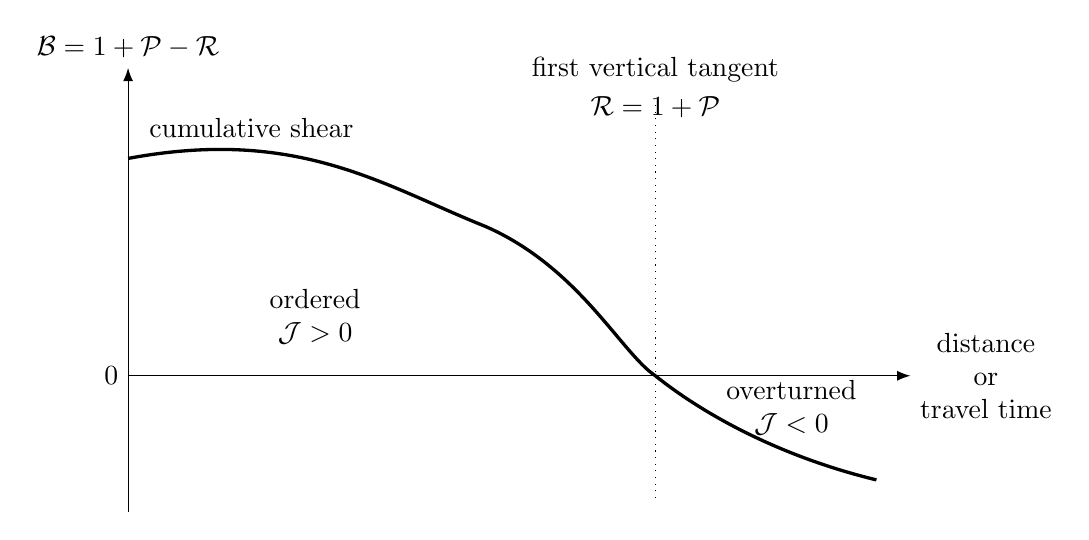
\begin{tikzpicture}[x=1.08cm,y=1.15cm,>=Latex]

  % Axes
  \draw[->] (0,0) -- (9.2,0)
    node[right,align=center] {distance\\or\\travel time};

  \draw[->] (0,-1.5) -- (0,3.4)
    node[above] {$\mathcal{B}=1+\mathcal{P}-\mathcal{R}$};

  \draw[dashed] (0,0.0) -- (9,0.0);
  \node[left] at (0,0) {$0$};

  % Main curve
  \draw[very thick]
    (0,2.4)
    .. controls (2.0,2.75) and (3.0,2.1) .. (4.2,1.65)
    .. controls (5.3,1.2) and (5.8,0.25) .. (6.2,0)
    .. controls (6.8,-0.45) and (7.7,-0.9) .. (8.8,-1.15);

  % First vertical tangent marker
  \draw[dotted] (6.2,-1.35) -- (6.2,3.0);

  % Centered annotations above the vertical dotted line
  \node[align=center] at (6.2,3.18)
    {first vertical tangent\\[2pt]$\mathcal{R}=1+\mathcal{P}$};

  % Region labels
  \node[align=center] at (2.2,0.65)
    {ordered\\$\mathcal{J}>0$};

  \node[align=center] at (7.8,-0.35)
    {overturned\\$\mathcal{J}<0$};

    % Shear annotations
  \node[above] at (1.45,2.52)
    {cumulative shear};

  % \draw[->,thin] (4.55,2.25) -- (5.15,1.05);
  % \node[above,align=center] at (4.45,2.31)
  %   {cumulative\\shear};

\end{tikzpicture}
\end{document}
